\section{Introduction to HTML5}
\begin{itemize}
    \item HTML: Hyper Text Markup Language
    \item It is a standard markup language.
    \item It is not programming language.
    \item Markup language uses standard words to define things within a document. 
    \item Browers don't display the html tags.
    \item HTML describes the structure of a web page. 
    \item It consists of a series of elements and those elements indicate to the web broser how to display the page.
    \item It is easy to learn.
\end{itemize}

\subsection{Why learn HTML?}
\begin{itemize}
    \item Create website for yourself or others (to sell them).
    \item Become a web designer or web developer.
    \item Understand the web.
    \item Make responsive and real-world websites.
\end{itemize}

\subsection{HTML vs HTML5}
\begin{itemize}
    \item HTML and HTML5 are similar.
    \item HTML is an older version, HTML5 is the latest version.
\end{itemize}

\subsection{CSS vs CSS3}
\begin{itemize}
    \item CSS and CSS3 same with the HTML and HTML5.
    \item CSS is the older version and CSS3 is the latest version.
\end{itemize}

%%%%%%%%%%%%%%%%%%%%%%%%%%%%%%%%%%%%%%%%%%%%%%%%%%%%%%
\section{Basic HTML document}
\begin{minted}[autogobble]{html}
    <!DOCTYPE html>
    <html>
        <head>
            <title> This is document title </title>
        </head>
        <body>
            <h1> My first heading </h1>
            <p> My first paragraph </h1>
        </body>
    </html>
\end{minted}
\begin{itemize}
    \item The first line is always \mintinline{html}{<!DOCTYPE html>}. 
        \begin{itemize}
            \item It must only appear once at the beggining.
        \end{itemize}
    
    \item The \mintinline{html}{<head>...</head>} contains the meta information of the page. Such as the title.
    \item The \mintinline{html}{<body></body>} tags defines and contains all the content that will be displayed in the web page.
    \item The \mintinline{html}{<h1></h1>} defines a header.
    \item The \mintinline{html}{<p></p>} defines a paragraph.
\end{itemize}

\subsection{HTML element syntax}
\begin{itemize}
    \item All HTML elements follow similar sintax:
        \begin{minted}[autogobble]{html}
            <tag-name> Content goes here </tag-name>
        \end{minted}
    
    \item The first tag is the opening tag, the second tag is the closing tag.
\end{itemize}

\subsection{Key points}
\begin{itemize}
    \item HTML always start with the \mintinline{html}{<!DOCTYPE html>}
    \item Begins with \mintinline{html}{<html>} and ends with \mintinline{html}{</html>}. Similar with body which starts with \mintinline{html}{<body>} and ends with \mintinline{html}{<body>}
    \item Never skip the end tag or closing tag.
    \item All html files must start with the .html extension.
\end{itemize}

%%%%%%%%%%%%%%%%%%%%%%%%%%%%%%%%%%%%%%%%%%%%%%%%%%%%%%
\section{Requirements to learn HTML5}
You will need a web browser and a code editor.
\begin{figure}[H]
    \centering
    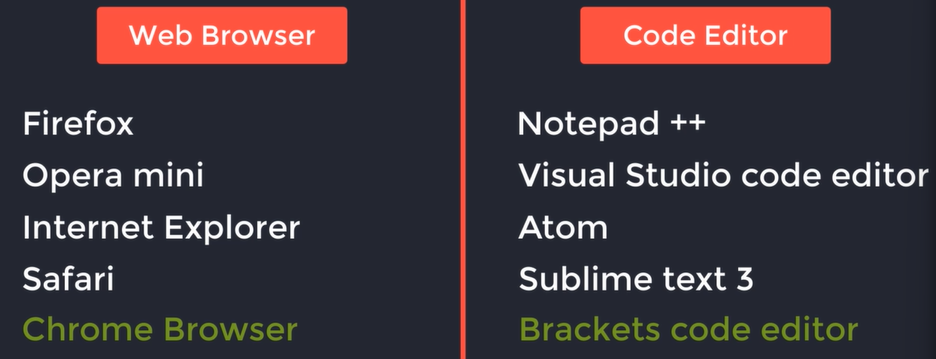
\includegraphics[width=\width\textwidth]{./figs/20220603225328.png}
    \caption{Requirements}
\end{figure}
